\documentclass[12pt,journal]{IEEEtran}

\usepackage[utf8]{inputenc}
\usepackage{graphicx}
\usepackage{amsmath}
\usepackage{amssymb}
\usepackage[]{algorithm2e}
\usepackage{float}

\begin{document}

\title{A weighted data representation based approach for manifold learning}
\author{A. Salgado - O. Lucía Quintero M.}
\maketitle

\begin{abstract}
    This work presents a detailed implementation of the local linear embeding
    algorithm from both a theoretical and practical approximation. In this work
    the dimensionality reduction is achieved by a two step procedure. First a
    weighted data representation based in $K$ nearest neighbors is calculated,
    and then a minimization of distance between the data representation and a
    low dimensionality configuration is conducted. Finally the resulting
    algorithm is tested on 3-dimensional manifolds.
\end{abstract}

\section{Introduction}


Exploratory data analysis and visualization are key issues in a lot of areas
in science. Gather knowledge about the structure and caracteristics of data
can lead to great improves in the process of solving problems in science. But a
good analysis of multidimensinal data can be really hard to achive, and the
consecuences of mistaken assumptions about the data properties can produce
dysfunctional solutions.

\vspace{0.25cm}

An approximation to solve these problems are dimensionality reduction techniques.
These methods provide a way to discover compact representations of
multidimensional datasets in a low dimensional space. This approaches allow the
analysis process to be carried out in an easier way and help to reduce the
probability of getting erroneous results.

\vspace{0.25cm}

However, there are still some issues related to the usage of these methods.
Assumptions like the use of euclidean distances as a measure in the
multidimensional space, implies that the data is homogeneous or isotropic, and
this is really often not the case in many real world datasets
\cite{homogeneous1}, \cite{homogeneous2}. Because of this, the usage of other
distance metrics is a good option to increase the performance of these approches
\cite{dist1}, \cite{dist2}.

\vspace{0.25cm}

An appropriate processing method for dimentionality reduction in the case of
a nonlinear approach can be manifold learning techniques \cite{manifold1},
\cite{manifold2}. This algorithms seek to generate nonlinear dimensionality
reductions by assuming that the data points are samples from a low dimensional
structure which is embedded in a multidimensional space and hence a simpler
representation can be constructed. \cite{manifold}

\vspace{0.25cm}

One example of a manifold learning algorithm is Local Linear Embeding (LLE)
\cite{lle}. This technique uses the fact that from a local perspective a
non-linear structure can be aproximated with an euclidean measure. Hence an
aproximation of a multidimensional manifold in a low dimensional space can be
conducted by representing small pieces, where the euclidean assumption can hold,
and then using these pieces together to get a reconstruction as similar as 
possible to the original manifold.

\vspace{0.25cm}

The objective of this work is to build a theoretical and practical develop of
the ideas used in the LLE algorithm to build a manifold learning method. For
this purpose the first part of the work will carafully describe each part of
the mathemathical backgound of the method, then the implementation details of
the algorithm are shown to prepare a results section, and finally some
conclusions are exposed.

\section{Theorical framework}

    As mention before, the problem that we are trying to solve is to find
    a low dimensional representation of points in a manifold that is in a high
    dimensional space. A theorical approximation of 
    the method is developed taking as staring point the description given in
    \cite{proof}. In this method two steps are considered. The
    first one is to find a way to represent each point in the original dataset as
    a linear combination of its $K$ nearest neighbors. This means that the
    objective is to find a set of weights that minimize the following
    expression

    \begin{equation*}
        \begin{aligned}
            \underset{w_{ij}}{\text{min}} \quad \sum_{i=1}^n & \lVert x_i - \sum_{j=1}^k w_{ij} N(x_i)_j \rVert^2 \\
            & \sum_{j=1}^k w_{ij} = 1
        \end{aligned}
    \end{equation*}

    Where $N(x_i)_j$ represents the $j$-th neighbor of the point $x_i$. The
    restriction is imposed to get a non trivial solution and ensure that
    the construction of the points is convex.\\

    This problem can be solved by optimizing an arbitrary case $i$. The first
    step is to define the neighborhood matrix of $x_i$, also a vector that will
    conatin the weights of the combination, and finally a special matrix $e$ that
    is filled with ones.

    \[
        V_i =
        \begin{bmatrix}
            |      &  |     &       & | \\
            N(x_i)_1 & N(x_i)_2 & \dots & N(x_i)_k \\
            |      &  |     &       & |
        \end{bmatrix}_{d \times k}
    \]
    \[
        W_i =
        \begin{bmatrix}
            w_{i1}\\
            w_{i2}\\
            \dots \\
            w_{ik}\\
        \end{bmatrix}_{k \times 1}
        \hspace{1cm}
        e =
        \begin{bmatrix}
        1\\
        1\\
        \dots\\
        1
        \end{bmatrix}_{k \times 1}
    \]

    With these tools the linear combinations of neighbors can be expressed as

    \begin{equation*}
        \sum_{j=1}^k w_{ij} N(x_i)_j = V_i W_i
    \end{equation*}

    Hence the problem can be rewritten as follows

    \begin{equation*}
            \underset{w_{ij}}{\text{min}} \lVert x_i - \sum_{j=1}^k w_{ij} N(x_i)_j \rVert^2
            =
            \underset{W_i}{\text{min}} \lVert x_i - V_i W_i \rVert^2
    \end{equation*}

    For the next step the objective is to represent $x_i$ as a vector operation.
    First a matrix in which each column is the $x_i$ point is constructed with
    the help of the $e$ vector

    \[
        x_i e^t =
        \begin{bmatrix}
            x_1 \\
            x_2 \\
            \dots \\
            x_d \\
        \end{bmatrix}_{d \times 1}
        \begin{bmatrix}
            1 & \dots & 1
        \end{bmatrix}_{1 \times k}
        =
        \begin{bmatrix}
            |   &       & | \\
            x_i & \dots & x_i\\
            |   &       & |
        \end{bmatrix}_{d \times k}
    \]\\

    Then using the fact that $W_i$ is used to construct a convex representation
    of the desired point, $x_i$ can be computed as

    \begin{equation*}
        x_i = x_i e^t W_i
    \end{equation*}

    Now the problem can be redefined in terms of matrix and vectors operations

    \begin{equation*}
        \begin{aligned}
            \underset{W_i}{\text{min}} \lVert x_i - V_i W_i \rVert^2
            &=
            \underset{W_i}{\text{min}} \quad \lVert x_i e^t W_i - V_i W_i \rVert^2\\
            &=
            \underset{W_i}{\text{min}} \quad \lVert (x_i e^t - V_i) W_i \rVert^2\\
            &=
            \underset{W_i}{\text{min}} \quad [(x_i e^t - V_i) W_i]^t [(x_i e^t - V_i) W_i]\\
            &=
            \underset{W_i}{\text{min}} \quad W_i^t(x_i e^t - V_i)^t (x_i e^t - V_i) W_i\\
        \end{aligned}
    \end{equation*}

    The next step is to define a matrix to simplify the objective function

    \begin{equation*}
        G = (x_i e^t - V_i)^t (x_i e^t - V_i)
    \end{equation*}

    With this matrix the problem can be rewritten as follows

    \begin{equation*}
            \underset{W_i}{\text{min}} \quad W_i^t(x_i e^t - V_i)^t (x_i e^t - V_i) W_i
            =
            \underset{W_i}{\text{min}} \quad W_i^t G W_i
    \end{equation*}

    An option to solve this problem are Lagrange multipliers. In order to use
    this method the restriction is redefined

    \begin{equation*}
        \sum_{j=1}^k w_{ij} = 1 = e^t W_i
    \end{equation*}

    Then a new objective function can be constructed

    \begin{equation*}
            \mathcal{L}(W_i, \lambda) = W_i^t G W_i - \lambda (e^t W_i - 1)
    \end{equation*}

    In order to optimize this function its derivative is calculated and then is
    set to 0

    \begin{equation*}
        \begin{aligned}
            \frac{\delta \mathcal{L}}{\delta W_i} &= 2 G W_i - \lambda e\\
            2 G W_i - \lambda e &= 0 \\
            2 G W_i &= \lambda e \\
            G W_i &= \frac{1}{2} \lambda e \\
            G^{-1} G W_i &= G^{-1} \frac{1}{2} \lambda e \\
            W_i &= \frac{1}{2} \lambda G^{-1} e \\
        \end{aligned}
    \end{equation*}

    At this point, if $\lambda$ is wrongly chosen, then the result would be a
    scaled version of the optimal value. Then, $\lambda$ can be chosen
    arbitrarily and after $W_i$ is computed, a rescale procedure can be
    conducted in order to satisfy the restriction.\\

    Hence, a good choice for the variable is $\lambda = 2$. This leads to the
    cancellation of the fraction and reduces the problem to find the solution of
    a linear system of equations

    \begin{equation*}
        \begin{aligned}
            W_i = \frac{1}{2} \lambda G^{-1} & e = G^{-1} e \\
            G W_i &= e \\
        \end{aligned}
    \end{equation*}

    This implies that matrix $G$ must be invertible, and there is no warranty
    of that. So, if that is the case, a solution is to recalculate $G$ as

    \begin{equation*}
        G \leftarrow G + \sigma I
    \end{equation*}

    where $\sigma$ is a small value.\\

    This procedure is used to find all of the weights values. Then these weights
    are used to define a configuration of points in a low dimensional space that
    is as similar as possible to the original dataset. The objective in this
    point is to minimize the following expression

    \begin{equation*}
        \begin{aligned}
            \underset{y}{\text{min}} \quad \sum_{i=1}^n & \lVert y_i - \sum_{j=1}^n w_{ij} N(y_i)_j \rVert^2 \\
            & YY^t = I
        \end{aligned}
    \end{equation*}

    Where

    \[
        Y =
        \begin{bmatrix}
            |   &  |  &       & |   \\
            y_1 & y_2 & \dots & y_n \\
            |   &  |  &       & |
        \end{bmatrix}_{p \times n}
        \hspace{0.5cm}
    \]

    To solve this problem, define

    \[
        \hspace{-0.5cm}
        W =
        \begin{bmatrix}
            |   &  |  &       & |   \\
            W_1 & W_2 & \dots & W_n \\
            |   &  |  &       & |
        \end{bmatrix}_{n \times n}
        where
        \hspace{0.25cm}
        W_i =
        \begin{bmatrix}
            0 \\
            w_1 \\
            \vdots \\
            w_k \\
            0 \\
        \end{bmatrix}_{n \times 1}
    \]

    Here $W_i$ is a vector that contains the value of the weight that correspond
    to the $j$ neighbor of $x_i$ in the corresponding position, and 0 anywhere
    else.\\

    Using this matrix the linear combinations of points can be calculated as

    \begin{equation*}
        \sum_{j=1}^k w_{ij} N(y_i)_j = Y W_i
    \end{equation*}\\

    Which means that the problem can be rewritten as

    \begin{equation*}
            \underset{y}{\text{min}} \quad \sum_{i=1}^n \lVert y_i - \sum_{j=1}^n w_{ij} N(y_i)_j \rVert^2
            =
            \underset{y}{\text{min}} \quad \sum_{i=1}^n \lVert y_i - Y W_i \rVert^2
    \end{equation*}

    \vspace{0.25cm}

    Now, just as before, the objective is to express $y_i$ as vectors operations.
    To achieve this, define

    \[
        I_i =
        \begin{bmatrix}
            0 \\
            \vdots \\
            1 \\
            \vdots \\
            0 \\
        \end{bmatrix}_{n \times n}
        \hspace{0.5cm}
    \]

    Which is a vector that has a $1$ in the $i$ position and $0$ anywhere else.
    With this new vector the problem can redefined as

    \begin{equation*}
            \underset{y}{\text{min}} \quad \sum_{i=1}^n \lVert y_i - Y W_i \rVert^2
            =
            \underset{y}{\text{min}} \quad \sum_{i=1}^n \lVert YI_i - Y W_i \rVert^2
    \end{equation*}

    \vspace{0.25cm}

    And now, since this expression is adding the norm of each vector in the
    matrix, the optimization problem can be rewritten to minimize the norm of
    the entire matrix

    \begin{equation*}
            \underset{y}{\text{min}} \quad \sum_{i=1}^n \lVert YI_i - Y W_i \rVert^2
            =
            \underset{Y}{\text{min}} \quad \lVert YI - Y W \rVert^2
    \end{equation*}

    This optimization problem can be solved as follows

    \begin{equation*}
        \begin{aligned}
            \lVert Y I - Y W \rVert^2 &= \lVert Y (I - W) \rVert^2\\
            &= Tr[(Y [I-W])^t (Y [I-W])]\\
            &= Tr[(I-W)^t Y^t Y (I-W)]\\
            &= Tr[(I-W)^t Y^t Y (I-W)]\\
            &= Tr[(I-W) (I-W)^t Y^t Y]\\
            &= Tr[Y (I-W) (I-W)^t Y^t]\\
        \end{aligned}
    \end{equation*}

    At this point define a matrix $M$ as

    \begin{equation*}
        M = (I-W) (I-W)^t
    \end{equation*}

    Redefine the optimization problem as

    \begin{equation*}
        \begin{aligned}
            \underset{Y}{\text{min}} \quad \lVert YI - Y W \rVert^2
            &=
            \underset{Y}{\text{min}} \quad Tr(Y M Y^t)\\
            &=
            \underset{Y}{\text{min}} \quad Tr(M Y^t Y)
        \end{aligned}
    \end{equation*}

    To solve this problem the Lagrange multipliers are used.

    \begin{equation*}
        \begin{aligned}
            \mathcal{L}(Y, \lambda) &= Tr( M Y^t Y) - \lambda (Y Y^t - I)\\
            \frac{\delta \mathcal{L}}{\delta W_i} &= Y M^t + Y M - 2 \lambda Y
        \end{aligned}
    \end{equation*}

    We know that matrix $M$ is symmetric

    \begin{equation*}
        \begin{aligned}
            M^t &= [(I-W) (I-W)^t]^t\\
                &= [(I-W)^t]^t (I-W)^t\\
                &= (I-W) (I-W)^t\\
                &= M
        \end{aligned}
    \end{equation*}

    Hence

    \begin{equation*}
        \begin{aligned}
            \frac{\delta \mathcal{L}}{\delta W_i} &= Y M^t + Y M - 2 \lambda Y\\
                                                  &= Y M + Y M - 2 \lambda Y\\
                                                  &= 2 Y M - 2 \lambda Y
        \end{aligned}
    \end{equation*}

    Finally, by setting this derivative to 0 the solution of the problem can
    be founded

    \begin{equation*}
        \begin{aligned}
            2 Y M - 2 \lambda Y &= 0 \\
                          2 Y M &= 2 \lambda Y \\
                            Y M &= \lambda Y \\
                            (Y M)^t &= (\lambda Y)^t \\
                            M^t Y^t &= Y^t \lambda \\
                            M Y^t &= \lambda Y^t \\
        \end{aligned}
    \end{equation*}

    Which is a eigenvector problem and can be solved with classical methods. 

\section{Algorithm implementation}

For the implementation of the method the programing language MATLAB \cite{matlab}
was used. This tool is specifically desing for matrix operations, which makes it
an appropriate option to address the problem in an easy way.

\vspace{0.25cm}

The Algorithm \ref{alg1} shows the seudo-code to compute a low
dimentional representation of a multidimensional manifold that is represented as
a matrix of points called data of dimensions $n$x$d$.

\begin{algorithm}
    $n$ = number of points\\
    $p$ = output dimensions\\
    $k$ = number of neighbors\\
    \vspace{0.5cm}
    $W$ = zeros($n$)\\
    \For{i in 1:n}{
        $x_i$ = data($i$)\\
        $k_i$ = get\_nearest\_neighbors($x_i$, $k$)\\
        $V_i$ = data($k_i$)\\
        $G$ = $(x_i e^t - V_i)^t (x_i e^t - V_i)$\\
        solve($G w_i = e$)\\
        $W(i)$ = $w_i$ / sum($w_i$)
    }
    \vspace{0.5cm}
    $M$ = $(I-W) * (I-W)^t$\\
    $V$ = get\_eigenvectors($M$)\\
    $Y$ = select\_smaller($p$, $V$)

    \vspace{0.5cm}

    \caption{Computation of low dimensional representation}
    \label{alg1}
\end{algorithm}

\section{Results}

The algorithm described in the previous secction was tested with 2 manifolds in
a 3 dimensional space. Figure \ref{swiss} shows a swiss roll dataset that
represents the manifold that the method is going to reduce, the resulting
2 dimensional dataset is shown in Figure \ref{swiss_res}.

\begin{figure}[H]
    \centering
    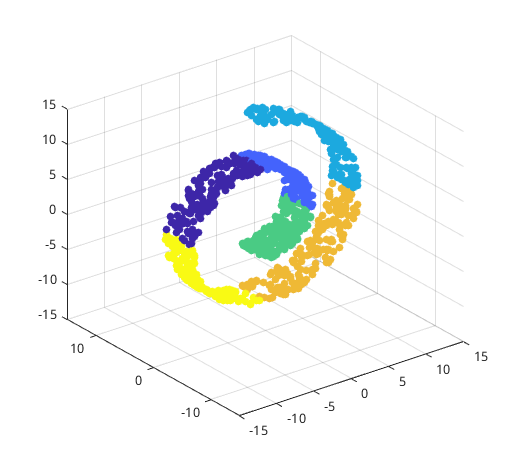
\includegraphics[width=0.8\linewidth]{images/swiss_roll.png}
    \caption{Swiss roll dataset}
    \label{swiss}
\end{figure}

\begin{figure}[H]
    \centering
    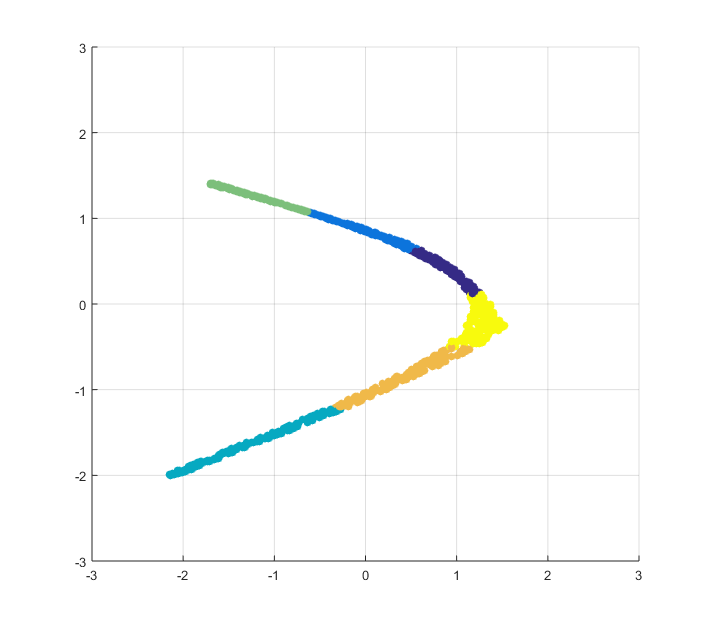
\includegraphics[width=0.7\linewidth]{images/swiss_roll_result.png}
    \caption{Swiss roll dataset reduced}
    \label{swiss_res}
\end{figure}

Finally in Figure \ref{sphere} a second manifold in form of a 3 dimensional
sphere is shown, the result of the method is shown in Figure \ref{sphere_res}
as a 2 dimensional configuration of points.

\begin{figure}[H]
    \centering
    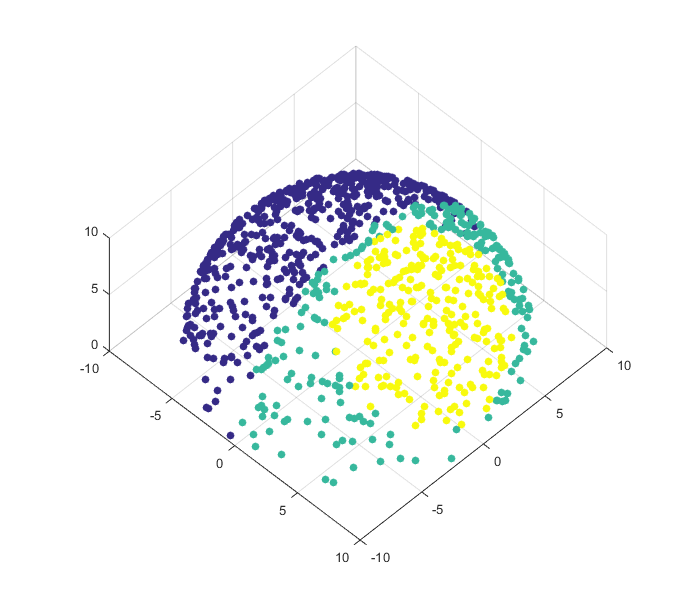
\includegraphics[width=0.8\linewidth]{images/sphere.png}
    \caption{Sphere dataset}
    \label{sphere}
\end{figure}

\begin{figure}[H]
    \centering
    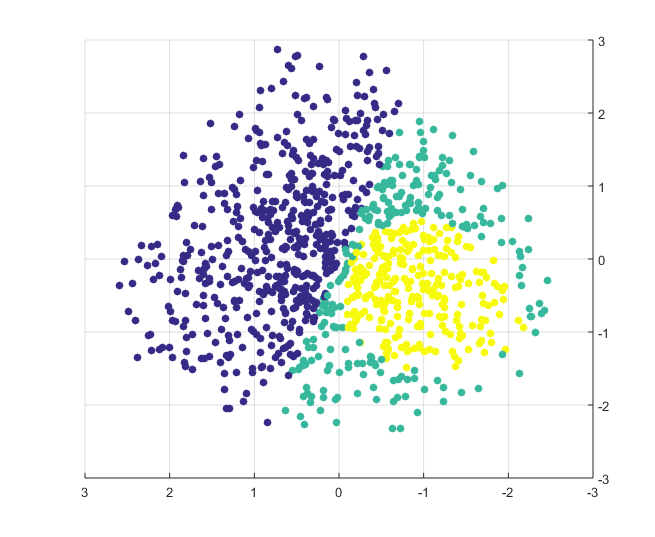
\includegraphics[width=0.8\linewidth]{images/sphere_result.png}
    \caption{Sphere dataset reduced}
    \label{sphere_res}
\end{figure}

\section{Conclusions}

In this work a theorical and practical develop of the local linear embeding
algorithm was described. During the process it was found that althought the
problems started with a quite complicated setup, the development of the problem
allowed to generate great simplifications that reduced the original problem to
just solve a linear system of equations and an eigenvector problem. These
simplifications made possible the creation of a relatively simple algorithm that
can detect low dimensional manifolds in multidimensional spaces. This statement
is supported in the results section where 3 dimensional manifolds were
simplified to dimension 2 but preserving the intrinsic structure of the original
dataset.

\bibliographystyle{unsrt}
\bibliography{Article_lle}

\end{document}
